\documentclass[12pt]{beamer}
\usepackage{../Estilos/BeamerMAF}
\usepackage{../Estilos/ColoresLatex}
%Sección para el tema de beamer, con el theme, usercolortheme y sección de footers
\usetheme{Frankfurt}
\usecolortheme{beaver}
%\useoutertheme{default}
\setbeamercovered{invisible}
% or whatever (possibly just delete it)
\setbeamertemplate{section in toc}[sections numbered]
\setbeamertemplate{subsection in toc}[subsections numbered]
\setbeamertemplate{subsection in toc}{\leavevmode\leftskip=3.2em\rlap{\hskip-2em\inserttocsectionnumber.\inserttocsubsectionnumber}\inserttocsubsection\par}
% \setbeamercolor{section in toc}{fg=blue}
% \setbeamercolor{subsection in toc}{fg=blue}
% \setbeamercolor{frametitle}{fg=blue}
\setbeamertemplate{caption}[numbered]

\setbeamertemplate{footline}
\beamertemplatenavigationsymbolsempty
\setbeamertemplate{headline}{}


\makeatletter
% \setbeamercolor{section in foot}{bg=gray!30, fg=black!90!orange}
% \setbeamercolor{subsection in foot}{bg=blue!30!yellow, fg=red}
% \setbeamercolor{date in foot}{bg=black, fg=white}
\setbeamertemplate{footline}
{
  \leavevmode%
  \hbox{%
  \begin{beamercolorbox}[wd=.333333\paperwidth,ht=2.25ex,dp=1ex,center]{section in foot}%
    \usebeamerfont{section in foot} \insertsection
  \end{beamercolorbox}%
  \begin{beamercolorbox}[wd=.333333\paperwidth,ht=2.25ex,dp=1ex,center]{subsection in foot}%
    \usebeamerfont{subsection in foot}  \insertsubsection
  \end{beamercolorbox}%
  \begin{beamercolorbox}[wd=.333333\paperwidth,ht=2.25ex,dp=1ex,right]{date in head/foot}%
    \usebeamerfont{date in head/foot} \insertshortdate{} \hspace*{2em}
    \insertframenumber{} / \inserttotalframenumber \hspace*{2ex} 
  \end{beamercolorbox}}%
  \vskip0pt%
}







\setbeamercolor{section in foot}{bg=antiquefuchsia, fg=white}
\setbeamercolor{subsection in foot}{bg=beaver, fg=white}
\setbeamercolor{date in foot}{bg=blue, fg=white}

\makeatletter
\setbeamertemplate{footline}
{
\leavevmode%
\hbox{%
\begin{beamercolorbox}[wd=.333333\paperwidth,ht=2.25ex,dp=1ex,center]{section in foot}%
  \usebeamerfont{section in foot} \insertsection
\end{beamercolorbox}%
\begin{beamercolorbox}[wd=.333333\paperwidth,ht=2.25ex,dp=1ex,center]{subsection in foot}%
  \usebeamerfont{subsection in foot}  \insertsubsection
\end{beamercolorbox}%
\begin{beamercolorbox}[wd=.333333\paperwidth,ht=2.25ex,dp=1ex,right]{date in head/foot}%
  \usebeamerfont{date in head/foot} \insertshortdate{} \hspace*{1.5em}
  \insertframenumber{} / \inserttotalframenumber \hspace*{2ex} 
\end{beamercolorbox}}%
\vskip0pt%
}
\makeatother
\usefonttheme{serif}
\setbeamercolor{frametitle}{bg=blond}
\resetcounteronoverlays{saveenumi}

\date{21 de abril de 2022}

\title{\large{Tema 4 - El átomo de hidrógeno}}
\subtitle{Funciones Especiales I}
\author{M. en C. Gustavo Contreras Mayén}

\begin{document}
\maketitle
\fontsize{14}{14}\selectfont
\spanishdecimal{.}

\section*{Contenido}
\frame[allowframebreaks]{\tableofcontents[currentsection, hideallsubsections]}

\section{Inicio con Funciones Especiales}
\frame{\tableofcontents[currentsection, hideothersubsections]}
\subsection{¿Qué son las funciones especiales?}

\begin{frame}
\frametitle{Comenzando con las funciones especiales}
Las funciones especiales en física matemática, son funciones solución de ecuaciones diferenciales ordinarias, que modelan diversos problemas en matemáticas, y son aplicadas en física para abordar problemas en astronomía, mecánica clásica, mecánica cuántica y fluidos, óptica, entre otras.
\end{frame}
\begin{frame}
\frametitle{Pensamiento}
Alberto Grünbaum del Departamento de Matemáticas de la Universidad de Berkeley, es uno de los mayores expertos mundiales en aplicaciones de funciones especiales y polinomios ortogonales, \pause en particular en probabilidad, procesos estocásticos, sistemas integrables, imagenología médica (tomografía computarizada), biomatemáticas y mecánica estadística, entre otros.
\end{frame}
\begin{frame}
\frametitle{El Dr. Alberto Grünbaum}
\begin{figure}
  \centering
  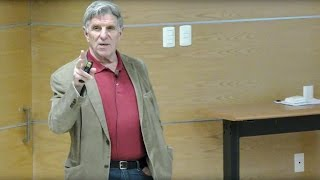
\includegraphics[scale=0.5]{Imagenes/Alberto_Grunbaum.jpg}
\end{figure}
\end{frame}
\begin{frame}
\frametitle{Pensamiento}
El Dr. Grünbaum expresó en una ocasión:
\\
\bigskip
\pause
\begin{quote}
\enquote{Las funciones especiales son para las matemáticas lo que las tuberías son para una casa: nadie quiere exhibirlas abiertamente, pero nada funciona sin ellas.}
\end{quote}
\end{frame}
\begin{frame}
\frametitle{Posturas encontradas}
También encontraremos otras posturas sobre las funciones especiales:
\pause
\begin{quote}
Las funciones (quizás mal llamadas) especiales de la Física Matemática no tienen nada de \enquote{especial}. En principio son tan \enquote{especiales} como las funciones trigonométricas o los logaritmos, aunque por supuesto son menos habituales.
\end{quote}
\end{frame}
\begin{frame}
\frametitle{Posturas encontradas}
Sigue la cita\footnote{Bravo, Y. S. (2006). \textit{Métodos Matemáticos Avanzados para Científicos e Ingenieros}, Colección Manuales UEX 48, Madrid, España}:
\pause
\begin{quote}
Un nombre más adecuado sería, sin duda, el de \emph{funciones útiles}. En todo caso, es lícito preguntarse por el motivo de estudiar estas funciones y sus propiedades.
\end{quote}
\end{frame}
\begin{frame}
\frametitle{Revisa el artículo}
Como una actividad de este tema, te pedimos que leas el siguiente artículo: 
\begin{thebibliography}{X}
\bibitem{Berry} Berry, M. (2001). \textit{Why are special functions special?}, Physics Today, \textbf{54} 4, 11, doi.org/10.1063/1.1372098.
\end{thebibliography}
Para que nos des tu opinión sobre lo que el autor expresa del tema de las funciones especiales.
\end{frame}

\section{¿Cómo se estudian?}
\frame{\tableofcontents[currentsection, hideothersubsections]}
\subsection{Método analítico}

\begin{frame}
\frametitle{Primera forma}
La primera forma de estudiar el conjunto de funciones especiales, es mediante el planteamiento de la ecuación diferencial.
\\
\bigskip
\pause
Para posteriormente aplicar lo revisado en los tres primeros temas del curso de MAF.
\end{frame}
\begin{frame}
\frametitle{Ruta a seguir}
Una posible ruta de trabajo es la siguiente:
\setbeamercolor{item projected}{bg=lava,fg=white}
\setbeamertemplate{enumerate items}{%
\usebeamercolor[bg]{item projected}%
\raisebox{1.5pt}{\colorbox{bg}{\color{fg}\footnotesize\insertenumlabel}}%
}
\begin{enumerate}[<+->]
\item EDP2H.
\item Separación de variables.
\item Método de Frobenius.
\item Segunda solución linealmente independiente.
\item Base completa.
\seti
\end{enumerate}
\end{frame}
\begin{frame}
\frametitle{Ruta a seguir}
\setbeamercolor{item projected}{bg=lava,fg=white}
\setbeamertemplate{enumerate items}{%
\usebeamercolor[bg]{item projected}%
\raisebox{1.5pt}{\colorbox{bg}{\color{fg}\footnotesize\insertenumlabel}}%
}
\begin{enumerate}[<+->]
\conti
\item Función generatriz.
\item Relaciones de recurrencia.
\item Paridad.
\item Ortogonalidad.
\item Formula de Rodrigues.
\seti
\end{enumerate}
\end{frame}
\begin{frame}
\frametitle{Ruta a seguir}
\setbeamercolor{item projected}{bg=lava,fg=white}
\setbeamertemplate{enumerate items}{%
\usebeamercolor[bg]{item projected}%
\raisebox{1.5pt}{\colorbox{bg}{\color{fg}\footnotesize\insertenumlabel}}%
}
\begin{enumerate}[<+->]
\conti
\item Ejercicios.
\item Ejemplos físicos.
\item Siguiente función especial.
\end{enumerate}
\end{frame}

%Ref. Marín (2014) - Métodos matemáticos
\subsection{Función generatriz}

\begin{frame}
\frametitle{Abordaje matemático}
En esta ocasión daremos inicio con una revisión que presentamos al concluir el tema de funciones especiales, ya que como lo veremos, el conjunto de expresiones que se estudian bajo un escenario particular, se pueden sintetizar en una única expresión que las genera.
\\
\bigskip
\pause
Por ello se le denomina \emph{ecuación generatriz}.
\end{frame}
\begin{frame}
\frametitle{Función generatriz}
La ecuación generatriz de las funciones especiales es una ecuación diferencial ordinaria de segundo orden lineal y homogénea:
\pause
\begin{align}
\dv{x} \bigg[ k(x) \, \dv{y}{x} \bigg] -  q(x) \, y + \lambda \, p(x) \, y = 0
\label{eq:ecuacion_01_01}
\end{align}
$\forall \, a < x < b$
\end{frame}
\begin{frame}
\frametitle{Función generatriz}
% \begin{align*}
% \dv{x} \bigg[ k(x) \, \dv{y}{x} \bigg] -  q(x) \, y + \lambda \, p(x) \, y = 0
% \end{align*}
Donde $k(x) > 0$, $q(x) \geq 0$ y $p(x) > 0$ son funciones definidas en el intervalo $[a, b]$ \pause y pueden tener dentro de este intervalo distintas características que se revisarán posteriormente; $\lambda$ es un parámetro.
\end{frame}

\subsection{Casos en la Ec. generatriz}

\begin{frame}
\frametitle{El por qué de la ec. generatriz}
La ec. (\ref{eq:ecuacion_01_01}) tiene el nombre de \emph{\textcolor{darkcerulean}{ecuación generatriz}}, \pause ya que para diferentes valores de $k(x)$, $q(x)$ y $p(x)$, se obtienen ecuaciones diferenciales cuyas soluciones son funciones especiales.
\end{frame}

\begin{frame}
\frametitle{Ec. de Bessel}
Con los valores:
\pause
\setbeamercolor{item projected}{bg=celadon,fg=black}
\setbeamertemplate{enumerate items}{%
\usebeamercolor[bg]{item projected}%
\raisebox{1.5pt}{\colorbox{bg}{\color{fg}\footnotesize\insertenumlabel}}%
}
\begin{multicols}{2}
\begin{enumerate}[<+->]
\item $k(x) = x$
\item $q(x) = \nu / x$
\item $p(x) = x$
\item $a = 0$
\item $b = x_{0}$
\item $\nu$ es un número cualquiera.
\end{enumerate}
\end{multicols}
\end{frame}
\begin{frame}
\frametitle{Ec. de Bessel}
Tendremos que:
\pause
\begin{align}
\dv{x} \bigg[ x \, \dv{y}{x} \bigg] -  \left( \lambda \, x  + \dfrac{\nu^{2}}{x} \right) \, y = 0
\label{eq:ecuacion_01_02}
\end{align}
\pause
Que al dividir entre $x$:
\pause
\begin{align}
\dfrac{1}{x} \, \dv{x} \bigg[ x \, \dv{y}{x} \bigg] -  \left( \lambda + \dfrac{\nu^{2}}{x^{2}} \right) \, y = 0
\label{eq:ecuacion_01_03}
\end{align}
\end{frame}
\begin{frame}
\frametitle{Ec. de Bessel}
Haciendo el cambio de variable: $\pderivada{x} = \sqrt{\lambda} \, x$, obtendremos:
\pause
\begin{align}
\begin{aligned}
\dfrac{1}{\pderivada{x}} \, \dv{\pderivada{x}} \bigg[ \pderivada{x} \, \dv{y}{\pderivada{x}} \bigg] &-  \bigg[ 1 - \dfrac{\nu^{2}}{x^{\, \prime \, 2}} \bigg] \, y = 0 \\[0.5em]
0 &< \pderivada{x} < \pderivada{x}_{0}
\end{aligned}
\label{eq:ecuacion_01_04}
\end{align}
\pause
Esta ecuación es conocida como \textbf{\textcolor{blue}{ecuación diferencial de Bessel}}.
\end{frame}
\begin{frame}
\frametitle{Aplicaciones de la ec. de Bessel}
Las soluciones a la ecuación de Bessel se denominan \textbf{funciones cilíndricas}, que se presentan en problemas de la física que involucran una geometría cilíndrica: condensadores cilíndricos, tubos embebidos con distintos potenciales o temperaturas, membranas circulares rígidas, etc.
\end{frame}
\begin{frame}
\frametitle{Geometría cilíndrica}
\begin{figure}
\centering
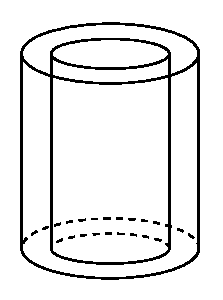
\includegraphics[scale=1.3]{Imagenes/cilindros_01.eps}
\end{figure}
\end{frame}
\begin{frame}
\frametitle{Ecuación asociada de Legendre}
Dejando los valores:
\pause
\setbeamercolor{item projected}{bg=celadon,fg=black}
\setbeamertemplate{enumerate items}{%
\usebeamercolor[bg]{item projected}%
\raisebox{1.5pt}{\colorbox{bg}{\color{fg}\footnotesize\insertenumlabel}}%
}
\begin{multicols}{2}
\begin{enumerate}[<+->]
\item $k(x) = 1 - x^{2}$
\item $q(x) = m^{2}/(1 - x^{2})$ con $m$ entero.
\item $p(x) = 1$
\item $a = -1$
\item $b = 1$
\end{enumerate}
\end{multicols}
\pause
La ec. (\ref{eq:ecuacion_01_01}) se convierte en:
\begin{align}
\dv{x} \bigg[ (1 - x^{2}) \, \dv{y}{x} \bigg] - \dfrac{m^{2}}{1 - x^{2}} \, y + \lambda \, y = 0
\label{eq:ecuacion_01_06}
\end{align}
\end{frame}
\begin{frame}
\frametitle{Ecuación asociada de Legendre}
\begin{align*}
\dv{x} \bigg[ (1 - x^{2}) \, \dv{y}{x} \bigg] &- \bigg[ \dfrac{m^{2}}{1 - x^{2}} \bigg] \, y + \lambda \, y = 0 \\[0.5em]
-1 &\leq x \leq 1
\end{align*}
\pause
que se conoce como \textcolor{darkmagenta}{ecuación diferencial asociada de Legendre}. \pause Las soluciones de esta ecuación se les denomina \textbf{\textcolor{darkpastelred}{polinomios asociados de Legendre}}.
\end{frame}
\begin{frame}
\frametitle{Ecuación asociada de Legendre}
La ec. (\ref{eq:ecuacion_01_05}) es un caso particular de la ec. (\ref{eq:ecuacion_01_06}), cuando $m = 0$.
\\
\bigskip
\pause
Las soluciones se presentan en problemas con geometría esférica.
\end{frame}
\begin{frame}
\frametitle{Ecuación ordinaria de Legendre}
Ahora con los valores:
\pause
\setbeamercolor{item projected}{bg=celadon,fg=black}
\setbeamertemplate{enumerate items}{%
\usebeamercolor[bg]{item projected}%
\raisebox{1.5pt}{\colorbox{bg}{\color{fg}\footnotesize\insertenumlabel}}%
}
\begin{multicols}{2}
\begin{enumerate}[<+->]
\item $k(x) = 1 - x^{2}$
\item $q(x) = 0$
\item $p(x) = 1$
\item $a = -1$
\item $b = 1$
\end{enumerate}
\end{multicols}
\pause
La ec. (\ref{eq:ecuacion_01_01}) toma la forma:
\begin{align}
\dv{x} \bigg[ (1 - x^{2}) \, \dv{y}{x} \bigg] + \lambda \, y = 0
\label{eq:ecuacion_01_05}
\end{align}
\end{frame}
\begin{frame}
\frametitle{Ecuación ordinaria de Legendre}
\begin{align*}
\dv{x} \bigg[ (1 - x^{2}) \, &\dv{y}{x} \bigg] + \lambda \, y = 0 \\[0.5em]
-1 &\leq x \leq 1
\end{align*}
\pause
que se conoce como \textcolor{cobalt}{ecuación diferencial ordinaria de Legendre}. \pause Las soluciones de esta ecuación se les denomina \textbf{\textcolor{darkcyan}{polinomios ordinarios de Legendre}}.
\end{frame}
\begin{frame}
\frametitle{Geometría esférica}
\begin{figure}
  \centering
  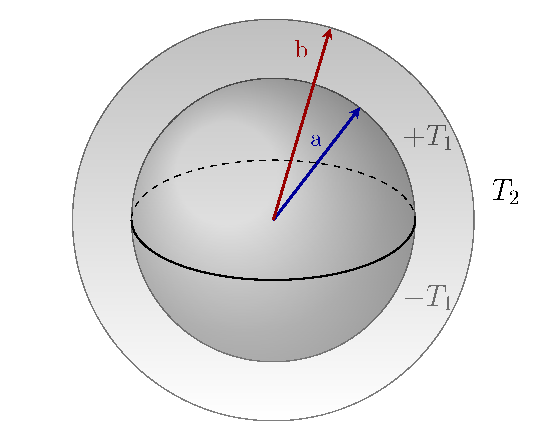
\includegraphics[scale=0.75]{Imagenes/esfera1.eps}
\end{figure}
\end{frame}
\begin{frame}
\frametitle{Otro ejemplo con geometría esférica}
\begin{figure}
  \centering
  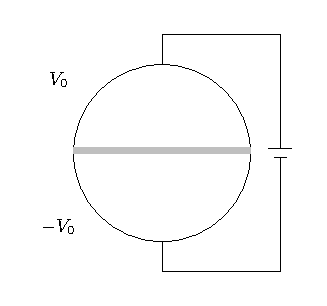
\includegraphics[scale=1]{Imagenes/Ejemplo_Esfera_03.eps}
\end{figure}
\end{frame}  
\begin{frame}
\frametitle{Ecuación de Laguerre}
Con los valores:
\pause
\setbeamercolor{item projected}{bg=cadmiumyellow,fg=black}
\setbeamertemplate{enumerate items}{%
\usebeamercolor[bg]{item projected}%
\raisebox{1.5pt}{\colorbox{bg}{\color{fg}\footnotesize\insertenumlabel}}%
}
\begin{multicols}{2}
\begin{enumerate}[<+->]
\item $k(x) = x \, \exp(-x)$
\item $q(x) = 0$
\item $p(x) = \exp(-x)$
\item $a = 0$
\item $b = \infty$
\end{enumerate}
\end{multicols}
\pause
La ec. (\ref{eq:ecuacion_01_01}) se convierte en:
\begin{align}
\dv{x} \bigg[ x \, \exp(-x) \, \dv{y}{x} \bigg] + \lambda \, \exp(-x) \, y = 0
\label{eq:ecuacion_01_08}
\end{align}
\end{frame}
\begin{frame}
\frametitle{Ecuación de Laguerre}
\begin{align*}
\dv{x} \bigg[ x \, &\exp(-x) \, \dv{y}{x} \bigg] + \lambda \, \exp(-x) \, y = 0 \\[0.5em]
&0 < x < \infty
\end{align*}
\pause
que se conoce como \textcolor{darkslateblue}{ecuación diferencial de Laguerre}.
\end{frame}
\begin{frame}
\frametitle{Ecuación de Laguerre}
Las soluciones de esta ecuación se les llama \textbf{\textcolor{denim}{polinomios de Laguerre}}, siendo las funciones especiales que se encuentran en el estudio del átomo de hidrógeno en su parte radial, bajo una geometría esférica.
\end{frame}
\begin{frame}
\frametitle{Ecuación generalizada de Laguerre}
En la mecánica cuántica se ocupa la \textbf{\textcolor{electricpurple}{ecuación generalizada de Laguerre}}:
\pause
\begin{align*}
\dv{x} \bigg[ x^{s+1} \, &\exp(-x) \, \dv{y}{x} \bigg] + \lambda \, x^{s} \, \exp(-x) \, y = 0 \\[0.5em]
&0 < x < \infty
\end{align*}
\pause
que se reduce a la ec. (\ref{eq:ecuacion_01_08}) con $s = 0$, las soluciones de esta ecuación son los llamados \textbf{\textcolor{fandango}{polinomios generalizados de Laguerre}}.
\end{frame}  
\begin{frame}
\frametitle{Ecuación de Hermite}
Usando los valores:
\pause
\setbeamercolor{item projected}{bg=beige,fg=black}
\setbeamertemplate{enumerate items}{%
\usebeamercolor[bg]{item projected}%
\raisebox{1.5pt}{\colorbox{bg}{\color{fg}\footnotesize\insertenumlabel}}%
}
\begin{multicols}{2}
\begin{enumerate}[<+->]
\item $k(x) = \exp(-x^{2})$
\item $q(x) = 0$
\item $p(x) = \exp(-x^{2})$
\item $a = -\infty$
\item $b = \infty$
\end{enumerate}
\end{multicols}
\pause
La ec. (\ref{eq:ecuacion_01_01}) se convierte en:
\begin{align}
\dv{x} \bigg[ \exp(-x^{2}) \, \dv{y}{x} \bigg] + \lambda \, \exp(-x^{2}) \, y = 0
\label{eq:ecuacion_01_07}
\end{align}
\end{frame}
\begin{frame}
\frametitle{Ecuación de Hermite}
\begin{align*}
\dv{x} \bigg[ \exp(-x^{2}) \, &\dv{y}{x} \bigg] + \lambda \, \exp(-x^{2}) \, y = 0 \\[0.5em]
&- \infty < x < \infty
\end{align*}
\pause
que se conoce como \textcolor{cadet}{ecuación diferencial de Hermite}. \pause Las soluciones de esta ecuación se les llama \textbf{\textcolor{camel}{polinomios de Hermite}}, que son la base para el estudio del oscilador armónico cuántico.
\end{frame}
\begin{frame}
\frametitle{Otras ecuaciones}
La ecuación generatriz de funciones especiales nos proporciona un primer conjunto de EDO2H.
\\
\bigskip
\pause
Debemos de considerar que también hay otro conjunto de ecuaciones que definen funciones especiales, que no necesariamente se obtienen de la ec. (\ref{eq:ecuacion_01_01}).
\end{frame}
\begin{frame}
\frametitle{Ecuación de Chebyshev tipo I}
La ecuación de Chebyshev de tipo I es:
\pause
\begin{align*}
(1 - x^{2}) \, \dv[2]{y}{x} - x \, \dv{y}{x} +  p^{2} \, y = 0
\end{align*}
\pause
Las soluciones a esta ecuación se conocen como \textbf{\textcolor{emerald}{polinomios de Chebyshev de tipo I}}. \pause Se encuentran en algoritmos de métodos numéricos computacionales.
\end{frame}
\begin{frame}
\frametitle{Ecuación de Chebycsev tipo II}
La ecuación de Chebyshev de tipo II es:
\pause
\begin{align*}
(1 - x^{2}) \, \dv[2]{y}{x} - 3 \, x \, \dv{y}{x} +  p(p + 2) \, y = 0
\end{align*}
\pause
Las soluciones a esta ecuación se conocen como \textbf{\textcolor{iceberg}{polinomios de Chebychev de tipo II}}. \pause Los polinomios de Chebyshev de tipo I y tipo II se encuentran relacionados entre sí.
\end{frame}
\begin{frame}
\frametitle{La ecuación hipergeométrica}
Estudiaremos la ecuación diferencial ordinaria hipergeométrica como punto de partida y encontraremos que habrá casos especiales o límite, en donde recuperamos otras funciones especiales.
\end{frame}
\begin{frame}
\frametitle{La ecuación hipergeométrica}
La \textbf{\textcolor{blue}{ecuación ordinaria hipergeométrica}} es:
\pause
\begin{align*}
x(x - 1) \, \stilde{y} + \big[ (1 + a + b) \, x - c \big] \, \pderivada{y} +  a \, b \, y = 0
\end{align*}
con $a, b, c \in \mathbb{R}$.
\end{frame}
\begin{frame}
\frametitle{La ecuación hipergeométrica confluente}
En el caso de la \textbf{\textcolor{red}{ecuación hipergeométrica confluente}} es:
\pause
\begin{align*}
x \, \stilde{y} + (c - x) \, \pderivada{y} +  a \, y = 0
\end{align*}
con $a, c \in \mathbb{R}$.
\end{frame}
\begin{frame}
\frametitle{Funciones de Gegenbauer}
Este tipo de funciones que se obtienen a partir de la serie hipergeométrica para los casos en donde ésta, es finita.
\\
\bigskip
\pause
Son la solución de la \textbf{\textcolor{iris}{ecuación diferencial de Gegenbauer}}, una generalización de los polinomios de Legendre.
\end{frame}
\begin{frame}
\frametitle{Precisión importante}
Las ecuaciones enlistadas que generan una función especial no son todas las que nos encontraremos en la física matemática.
\\
\bigskip
\pause
El punto importante es enfocarse en la metodología de estudio de las funciones especiales, ya que con ella, podremos desarrollar las soluciones, caracterizarlas y ocuparlas en la resolución de un problema en específico.
\end{frame}


\subsection{Método con la física}

\begin{frame}
\frametitle{Método con aplicación}
Con esta manera de estudio, se plantea de inicio un problema físico que permitirá entonces deducir una serie de elementos necesarios que se \enquote{conectan} con el desarrollo: por qué un determinado valor para una constante de separación, por ejemplo.
\end{frame}
\begin{frame}
\frametitle{La física como primer elemento}
El estudiar un fenómeno físico nos llevará a plantear una EDP como modelo matemático, por lo que se continua el análisis de la función especial como en el listado anterior.
\end{frame}
\begin{frame}
\frametitle{¿Cuál es la ventaja de uno método del otro?}
Estando en el sexto semestre de la carrera, es necesario abordar el estudio de las funciones especiales siempre con un ejemplo que permita enlazar lo que vemos en otras asignaturas, con este estudio de la física matemática.
\end{frame}
\begin{frame}
\frametitle{Varios caminos para llegar a lo mismo}
Veremos que habrá varias funciones especiales que permitirán llegar a un mismo planteamiento, en lo que refiere a la EDP, pero ocupando distintas áreas de la física.
\\
\bigskip
\pause
Esto nos pone en evidencia la relevancia de las funciones especiales.
\end{frame}
% \begin{frame}
% \frametitle{Punto importante}
% Cabe señalar que las funciones especiales que revisaremos en este curso de MAF, \emph{NO} son todas las funciones que se pueden encontrar en la física matemática, así como las transformadas integrales.
% \end{frame}
\begin{frame}
\frametitle{Aportación para un estudio posterior}
Lo que buscamos también es que cuenten con las habilidades de trabajo para revisar una función especial muy particular con la que se encuentren, y puedan entonces resolver el problema al que se enfrentan.
\end{frame}

\section{Objetivos del Tema 4}
\frame{\tableofcontents[currentsection, hideothersubsections]}
\subsection{El átomo de hidrógeno}

\begin{frame}
\frametitle{Iniciando el Tema 4}
El Tema 4: Dará inicio con el estudio (\emph{breve}) del átomo de hidrógeno como ejemplo clásico de la mecánica cuántica.
\\
\bigskip
\pause
La naturaleza del problema nos sugiere ocupar un sistema coordenado esférico.
\end{frame}
\begin{frame}
\frametitle{Objetivos}
Al terminar el Tema 4 se espera que el alumno:
\setbeamercolor{item projected}{bg=ao,fg=white}
\setbeamertemplate{enumerate items}{%
\usebeamercolor[bg]{item projected}%
\raisebox{1.5pt}{\colorbox{bg}{\color{fg}\footnotesize\insertenumlabel}}%
}
\begin{enumerate}[<+->]
\item Utilice el operador momento angular como elemento necesario para construir la solución del problema del átomo de hidrógeno, en su parte angular.
\item Estudiará los armónicos esféricos como funciones propias del operador momento angular.
\seti
\end{enumerate}
\end{frame}
\begin{frame}
\frametitle{Objetivos}
\setbeamercolor{item projected}{bg=ao,fg=white}
\setbeamertemplate{enumerate items}{%
\usebeamercolor[bg]{item projected}%
\raisebox{1.5pt}{\colorbox{bg}{\color{fg}\footnotesize\insertenumlabel}}%
}
Revisará las propiedades de las soluciones de:
\begin{enumerate}[<+->]
\conti
\item La ecuación diferencial asociada de Legendre.
\item La ecuación diferencial ordinaria de Legendre.
\end{enumerate}
\pause
Recuperando la solución de la parte angular del problema del átomo de hidrógeno.
\end{frame}

\section{Evaluación del Tema}
\frame{\tableofcontents[currentsection, hideothersubsections]}
\subsection{Ejercicios del Tema 4}

\begin{frame}
\frametitle{Lista de ejercicios}
En la clase del día 26 de abril se presentará la lista de ejercicios a resolver del Tema 4.
\\
\bigskip
\pause
La entrega queda programada para el jueves 19 de mayo a las 6 pm vía Moodle.
\end{frame}
\begin{frame}
\frametitle{Lista de enunciados para el segundo examen}
En la misma sesión del 26 de abril se presentará la lista de 10 enunciados para la parte que corresponde del Segundo Examen del curso.
\\
\bigskip
\pause
Se indicará en su momento, cuáles serán los 6 ejercicios que quedarán incluidos.
\end{frame}

% \begin{frame}
% \frametitle{Ejercicios a cuenta}
% La distribución de ejercicios es la siguiente:
% \pause
% \renewcommand{\arraystretch}{1.25}
% \begin{table}
% \centering
% \begin{tabular}{l c c}
% Material & Semanales & Opcionales \\ \hline
% Lectura Berry & 1 &  \\ \hline
% Armónicos esféricos  & 2 & 1 \\ \hline
% Ec. asociada Legendre & 2 & 1 \\ \hline    
% Ec. ordinaria Legendre & 2 & 1 \\ \hline    
% Teorema de adición & 1 & 1
% \end{tabular}
% \end{table}
% \end{frame}

% \subsection{Examen Tarea}

% \begin{frame}
% \frametitle{Entrega del examen tarea 3}
% En la sesión del 3 de diciembre se entregarán los enunciados del examen tarea 4, \pause para enviar la solución el día 19 de diciembre.
% \end{frame}

\section{Cronograma de trabajo}
\frame{\tableofcontents[currentsection, hideothersubsections]}
\subsection{Trabajo por semana}

\begin{frame}
\frametitle{Distribución de tiempos}
Para cubrir los materiales de trabajo del Tema 4, se presenta la siguiente distribución de tiempos:
\end{frame}
\begin{frame}
\frametitle{Distribución de tiempos}
\setbeamercolor{item projected}{bg=coquelicot,fg=white}
\setbeamertemplate{enumerate items}{%
\usebeamercolor[bg]{item projected}%
\raisebox{1.5pt}{\colorbox{bg}{\color{fg}\footnotesize\insertenumlabel}}%
}
\begin{enumerate}[<+->]
\item Semana 9: Lectura de Berry y átomo de hidrógeno.
\item Semana 10: Armónicos esféricos y Ec. asociada de Legendre.
\item Semana 11 y la sesión del 12 de mayo (Semana 12): Ec. ordinaria de Legendre y Teorema de adición.
\end{enumerate}
\end{frame}
% \begin{frame}
% \frametitle{Sesiones síncronas de trabajo}
% Se programan las siguientes sesiones de trabajo:
% \begin{itemize}[<+->]
% \item Martes 16 y viernes 19 de noviembre.
% \item Miércoles 24 y viernes 26 de noviembre.
% \item Miércoles 1 y viernes 3 de diciembre.
% \item Lunes 6 de diciembre.
% \end{itemize}
% \end{frame}
\end{document}